\par The usual neural network problem formulation involves predicting values based on existing observations. When the output domain is a continuous space, it becomes a regression problem. Prediction of discrete values, on the other hand, is called classification \cite{D2l}.

\par In the following, we consider a independent variable $\mathrm{x}$ of input features and some targets $\mathrm{y}$ dependent on $\mathrm{x}$ in an approximately linear way. 
\par In its simplest form, $\mathrm{x}$ is unidimensional variable and dependence between $\mathrm{x}$ and $\mathrm{y}$ is approximated by the relation $\mathrm{y}=\alpha \mathrm{x} + \beta$. Our aim is to find $\alpha$ and $\beta$ that best fit a set of $n$ observations of the behavior of $y^(i)$ with respect to the input $x^(i)$, $(x^{(i)}, y^{(i)})_{i=\overline{1,n}}$. We are trying to find the optimal parameters that minimize the error $|y^{(i)}-\alpha x^{(i)} - \beta|$ across all observations --- see Figure \ref{FigLinReg2D}.

\par Let's define the cummulative error $err(\alpha, \beta)=\sum_{i=1}^{n}{\left| \alpha x^{(i)}+\beta-y^{(i)} \right| ^2}
= \sum_{i=1}^n{(x_{(i)})^2} \alpha^2 + n \beta^2 + \sum_{i=1}^n{(y_{(i)})^2} 
+ 2\sum_{i=1}^n{x_{(i)}} \alpha\beta - 2\sum_{i=1}^n{x_{(i)}}{y_{(i)}} \alpha 
- 2\sum_{i=1}^n{y_{(i)}} \beta$. The function reaches its critical point in $(\alpha^\star, \beta^\star)$ which cancels the gradient:
$\nabla err = 0 \leftrightarrow (\frac{\partial err}{\partial \alpha}, \frac{\partial err}{\partial \beta})=0 \leftrightarrow$
$$
\begin{cases}
2\sum_{i-1}^n{(x^{(i)})^2}\alpha +2\sum_{i-1}^n{x^{(i)}}\beta - 2\sum_{i-1}^n{x^{(i)}y^{(i)}} = 0 \\
2\sum_{i-1}^n{x^{(i)}}\alpha + 2 n \beta - 2\sum_{i-1}^n{y^{(i)}} = 0.
\end{cases}
$$
The system can be written in matrix form as 
$$
\begin{bmatrix}
\sum_{i-1}^n{(x^{(i)})^2} & \sum_{i-1}^n{x^{(i)}} \\
\sum_{i-1}^n{x^{(i)}} & n
\end{bmatrix} \begin{bmatrix}
\alpha \\ \beta
\end{bmatrix} = \begin{bmatrix}
    \sum_{i-1}^n{x^{(i)}y^{(i)}} \\
    \sum_{i-1}^n{y^{(i)}}
\end{bmatrix}.
$$
With the notation $X^T=\begin{bmatrix} x^{(1)} & x^{(2)} &  \dots & x^{(n)} \\ 1 & 1 & \dots & 1 \end{bmatrix}$ and $Y^T=\begin{bmatrix}y^{(1)} & y^{(2)} & \dots & y^{(n)} \end{bmatrix}$, we are left with the nice equation $X^T X \begin{bmatrix}
\alpha \\ \beta \end{bmatrix} = X^T Y$, whose solution is 
$$\begin{bmatrix}\alpha \\ \beta \end{bmatrix} = (X^T X)^{-1} X^T Y,$$
The described approach is called the Least Square Method (LSM) \cite{linregreview}, which focuses on minimizing the square of the fitting errors for each data in the system.

\begin{figure}[htbp]
	\centering
		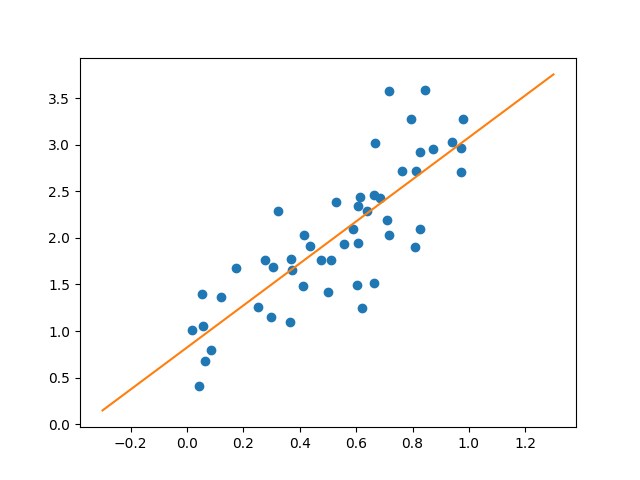
\includegraphics[scale=0.5]{figures/lin_reg_2d.png}
	\caption{Linear regression example in 2D space, with $\alpha=2, \beta=1$}
	\label{FigLinReg2D}
\end{figure}

This method can be extended to multivariate linear regression \cite{linregreview}, where each observation $x^{(i)}$ consists of multiple features $x^{(i)}_1,\ldots,x^{(i)}_m$ and we are finding the values $\beta=(\beta_0,\ldots,\beta_m)$ that minimize $\beta_0 + \beta_1 x^{(1)}+\ldots+\beta_m x^{(m)}$. By taking $X^T=\begin{bmatrix}
x^{(1)}_1 & x^{(2)}_1 & \ldots & x^{(n)}_1 \\
\vdots & \vdots & \ddots & \vdots \\
x^{(1)}_m & x^{(2)}_m & \ldots & x^{(n)}_m \\
1 & 1 & \ldots & 1 
\end{bmatrix}$, the previous relation $\beta = (X^T X)^{-1}X^T Y$ holds true, as long as $ (X^T X)$ is invertible. A singular matrix would suggest that the variables $x$ may not be linearly independent. There may exist a hyperplane of lower order that contains them and allows for infinite regression possibilities (for example, all $x^{(i)}$ are located in the same point in a 2D space through which can pass an infinity of lines, or on a line in 3D space).

Obviously the linear regression is designed to only find almost linear relations between data. One famous example is the XOR function \ref{FigXorLin}. Attempting to obtain a prediction by linear regression would lead to a function that uniformly averages the expected output values, and thus it is said that the values are linearly inseparable \cite{xorexample}. Another drawback of this method is the requirement to compute the inverse of the matrix in order to solve the system, which can prove computationally expensive. This opens up the door for faster iterative and potentially more general approaches, like the gradient descent, which will be discussed later in this thesis.

\begin{figure}[htbp]
	\centering
		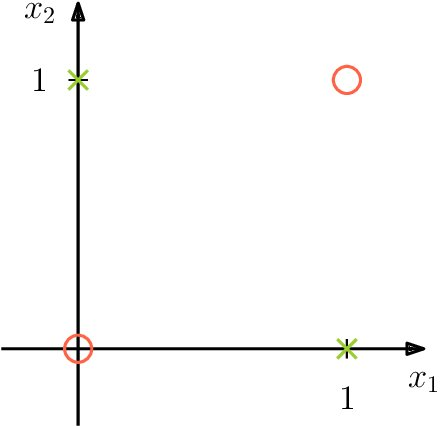
\includegraphics[scale=1]{figures/xor_lin.jpg}
	\caption{The XOR function cannot be predicted by a linear regression model \cite{xorexample}}
	\label{FigXorLin}        
\end{figure}




\par However, we can derive from this method a recurrent aspect in optimization problems: the concept of loss function. A loss function is a function $\mathcal{L}(\mathrm{y}, \mathrm{y^\star})$ destined to 
measure the reliability of our prediction by comparing the real reference values with the predicted output. Minimizing the loss function is associated with a better prediction \cite{losssurvey}. The loss function 
$err$ used by LSM is an example of loss function. Other common regression loss functions are Mean Absolute Error (MAE) or $\mathcal{L}_1$ loss, $\mathcal{L}_{MAE} = \frac{1}{n}\sum_{i=1}^n{\left| y_i - y_i^\star \right|}$, the Mean Squared Error (MSE), or $\mathcal{L}_2$ loss, $\mathcal{L}_{MAE} = \frac{1}{n}\sum_{i=1}^n{\left| y_i - y_i^\star \right|^2}$, or the Huber loss, which combines the previous two functions by exploiting the fact that MAE is good for large errors and MSE is suitable for smaller residuals \cite{losssurvey}.


\par A widely adopted approach to fight linearity in predictions is to pass the outputs $\mathrm{y}^\star$ to a (non-linear) function called an activation function \cite{activsurvey}. They are meant to increase the ability of the solution to find more sophisticated relations in the processed data. Their role will be emphasized when we will talk about neural network layers. By chaining two linear prediction functions $f_1$ and $f_2$ with no activation (or, synonymously, linear activation), the result $f_1 \circ f_2$ is also linear. However, by applying a non-linear activation $f_a$ to $f_1$ before plugging its results into $f_2$, the resulted application $f_1 \circ f_a \circ f_2$ is no longer linear in terms of the input $\mathrm{x}$. Table \ref{Activations} contains a list of popular activation functions \cite{activsurvey}.


\begin{table}[htbp]
\begin{center}
\begin{tabular}
{|p{120pt}|p{120pt}|}
\hline
 Name  &  Formula\\
\hline Tanh & $(e^{2x}-1)/(e^{2x}+1)$ \\ 
\hline ReLU & $\max(0, x)$ \\ 
\hline LeakyReLU & $ x, \text{if} \ x \geq 0, \text{else} \ \alpha x $ \\ 
\hline Sigmoid & $(1+e^{-x})^{-1}$ \\ 
\hline Swish & $x \cdot \textit{sigmoid}(x)$ \\ 
\hline
\end{tabular}
\end{center}
\caption{Common activation functions \cite{activsurvey}}
\label{Activations}
\end{table}

%\marginpar{\textcolor{green}{eu zic ca acestea sunt functii de activare (in tabelul 2.1, nu fc de loss)}} % solved (copy paste issues)
The choice for loss and activation functions is solely dependent on the problem \cite{losssurvey}. They can dictate the eligibility of the solution and convergence rate. Like LeakyReLU, most functions allow customizing their parameters (called hyperparameters) and in most machine learning frameworks come with multiple variants (like the scaled sigmoid, hard sigmoid etc.) \cite{activsurvey}, \cite{actfcomp}.